% File: team_report.tex
\documentclass[letterpaper]{article} % DO NOT CHANGE THIS
\usepackage{aaai24}  % DO NOT CHANGE THIS
\usepackage{times}             % DO NOT CHANGE THIS
\usepackage{helvet}            % DO NOT CHANGE THIS
\usepackage{courier}           % DO NOT CHANGE THIS
\usepackage[hyphens]{url}      % DO NOT CHANGE THIS
\usepackage{graphicx}          % DO NOT CHANGE THIS
\urlstyle{rm}                % DO NOT CHANGE THIS
\def\UrlFont{\rm}            % DO NOT CHANGE THIS
\usepackage{natbib}          % DO NOT CHANGE THIS
\usepackage{caption}         % DO NOT CHANGE THIS
\frenchspacing               % DO NOT CHANGE THIS
\setlength{\pdfpagewidth}{8.5in}  % DO NOT CHANGE THIS
\setlength{\pdfpageheight}{11in}  % DO NOT CHANGE THIS
\pdfinfo{
/TemplateVersion (2024.1)
}

\title{Training a Lightweight ResNet Implementation on CIFAR-10}
\author{
    Daesung Jin, Yongjae Chung
}
\affiliations{
    New York University\\
    \123123@nyu.edu, yc3028@nyu.edu
}

\begin{document}
\maketitle

% \begin{abstract}
% This project report presents our approach to building an accurate and efficient residual neural network that performs image classification on the CIFAR-10 dataset, under the constraint of 5 million parameters. We explore a lightweight ResNet architecture enhanced with advanced data augmentation techniques, hyperparameter adjustments, and teacher-student techniques. We describe our methodology, architecture design, training process, and empirical findings. Our final model achieved a test accuracy of \textbf{XX\%} and consists of \textbf{YY} parameters.
% \end{abstract}

\section{Abstract}
This project report presents our approach to building an accurate and efficient residual neural network that performs image classification on the CIFAR-10 dataset, under the constraint of 5 million parameters. We explore a lightweight ResNet architecture enhanced with advanced data augmentation techniques, hyperparameter adjustments, and teacher-student techniques. We describe our methodology, architecture design, training process, and empirical findings. Our final model achieved a test accuracy of \textbf{XX\%} and consists of \textbf{YY} parameters.

% \section{Team Members}
% \begin{itemize}
%     \item Daesung Jin
%     \item Yongjae Chung
% \end{itemize}

\section{Project Overview and Findings}
We developed a custom ResNet-inspired model tailored for CIFAR-10. Our work consisted of:
\begin{itemize}
    \item A modified residual block and ResNet architecture with adaptive average pooling.
    \item Integration of an advanced augmentation pipeline based on AutoAugment, random flipping, and Cutout.
    \item Experimentation with hyperparameter tuning, including adjustments in filter size, kernal size and pooling size.
    \item Regularization such as a dropout layer and weight decay.
    \item Implementation of unstructured pruning using PyTorch’s pruning utilities.
    \item Implementation of learning rate scheduling, early stopping, and a train-validation split to reduce overfitting.
\end{itemize}

Our experiments showed that our initial local validation accuracy reached around 85\%, our competition test data accuracy dropped to about 70\%, indicating overfitting. With a proper validation split and early stopping, we managed to reduce overfitting. Incremental improvements were observed with added dropout and weight decay (increasing accuracy from approximately 83\% to 85\%). Minimal augmentation (crop, horizontal flip, normalization) achieved around 85\%, whereas adding AutoAugment policy did not further improve performance. Increasing weight decay from $1\times10^{-4}$ to $5\times10^{-4}$ also showed incremental improvement.

\section{Methodology}
\subsection{Model Architecture}
Our architecture is a lightweight ResNet variant with four residual blocks of increasing channels: \texttt{[64, 128, 256, 512]}. Each block uses two \texttt{3$\times$3} convolutions, batch normalization, and ReLU activations, with skip connections implemented via 1$\times$1 convolutions when necessary. Downsampling is performed with stride-2 convolutions. We experimented with modifying the filter size in the initial layer (e.g., using 7$\times$7 or 5$\times$5 filters) to capture more spatial context. Our experiments showed that a 7$\times$7 filter resulted in a validation accuracy of 83.66\%, while a 5$\times$5 filter achieved 83.55\%, resulting in the 3$\times$3 filter performing the best (85.3\%).

\subsection{Data Augmentation Pipeline}
We applied a multi-step augmentation process, to provide more generalization to our model:
\begin{itemize}
    \item \textbf{AutoAugment (CIFAR-10 policy):} Utilized learned transformation policies to increase data diversity.
    \item \textbf{Random Cropping and Horizontal Flipping:} Introducing spatial variability.
    \item \textbf{Color Jittering and Cutout:} Altered photometric properties and masked out random image regions to improve generalization.
    \item \textbf{Normalization:} We normalized images using CIFAR-10-specific mean and standard deviation: (TODO CITATION)
    \begin{itemize}
        \item Mean: [0.4914, 0.4822, 0.4465]
        \item Std: [0.247, 0.243, 0.261]
    \end{itemize}
\end{itemize}

Initially, we employed a relatively aggressive augmentation strategy. However, we later reduced the augmentation to a lighter-weight version (horizontal flip, AutoAugment, crop, normalization) to establish a baseline.

\subsection{Training Strategy and Regularization}
Our training strategy includes:
\begin{itemize}
    \item \textbf{Optimizer:} Adam with an initial learning rate of 0.001. Later changed to SGD with initial learning rate of 0.1.
    \item \textbf{Learning Rate Scheduling:} A StepLR scheduler decays the learning rate by a factor of 0.1 every 10 epochs.
    \item \textbf{Early Stopping:} Implemented with a patience of 3 epochs based on validation loss.
    \item \textbf{Regularization:} We introduced dropout (with $p=0.5$) after the pooling layer and added weight decay ($1\times10^{-4}$ initially, later increased to $5\times10^{-4}$) in the optimizer. These modifications improved our validation accuracy to around 83-84\% and eventually to 85\% with minimal augmentation.
\end{itemize}

\subsection{Pruning and Fine-tuning}
We applied unstructured L1 pruning to \texttt{Conv2d} and \texttt{Linear} layers, targeting 20\% sparsity. Although this masked many weights to zero, the total parameter count remained unchanged as reported by \texttt{torchsummary}. Therefore we did not proceed this with approach, as our initial plan was to make a deeper ResNet and prune, but with this limitation, we were not able to reduce parameters.

\subsection{Dataset Splitting and Validation}
To address overfitting, we split the CIFAR-10 training data into 90\% training and 10\% validation sets \textit{before} applying data augmentation. This helped ensure that the validation set remained uncontaminated by aggressive augmentations and provided a reliable estimate of the model’s generalization performance.

\subsection{Challenges and Insights}
Our experiments revealed several insights:
\begin{itemize}
    \item Adjusting the filter size and pooling strategy had modest effects on performance.
    \item Overfitting was evident when the model achieved near-zero training loss but a plateaued validation loss.
    \item Incorporating early stopping, dropout, and weight decay was crucial to mitigating overfitting.
    \item Minimal augmentation (crop, horizontal flip, normalization) performed well, while additional augmentation via AutoAugment did not yield significant improvements.
    \item Increasing the weight decay value from $1\times10^{-4}$ to $5\times10^{-4}$ provided further gains.
\end{itemize}

\section{Results}
Our final model achieved:
\begin{itemize}
    \item \textbf{Validation Accuracy:} XX\%
    \item \textbf{Test Accuracy:} XX\%
    \item \textbf{Trainable Parameters:} YY million
\end{itemize}

\begin{figure}[h]
\centering
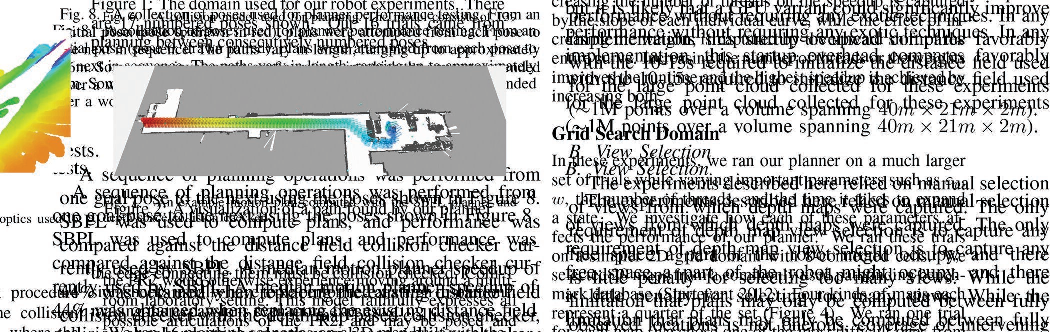
\includegraphics[width=0.9\linewidth]{AuthorKit24-4/CameraReady/LaTeX/figure2.pdf}
\caption{Training and validation loss curves over 30 epochs.}
\end{figure}

\begin{figure}[h]
\centering
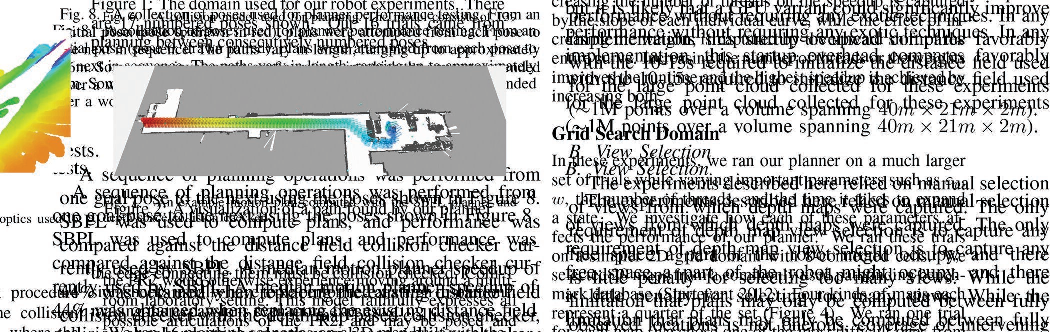
\includegraphics[width=0.9\linewidth]{AuthorKit24-4/CameraReady/LaTeX/figure2.pdf}
\caption{Examples of training images after augmentation (AutoAugment + Cutout).}
\end{figure}

Notably, while our local test set achieved approximately 85\% accuracy, the competition test data accuracy was only around 70\%, indicating that overfitting was a significant concern. This motivated our adoption of a train-validation split and early stopping, which helped reduce overfitting and improve generalization.

\section{Conclusion}
This project demonstrates that careful tuning of the ResNet architecture, combined with advanced data augmentation and regularization techniques, can yield competitive performance on CIFAR-10 under strict parameter constraints. While unstructured pruning helps reduce redundant weights, future work may explore structured pruning or alternative architectures (e.g., MobileNet or EfficientNet) for further parameter reduction.

Potential future directions include:
\begin{itemize}
    \item Structured pruning for actual model compression.
    \item Progressive augmentation strategies.
    \item Incorporation of mixup or label smoothing.
    \item Exploration of lightweight architectures under the same constraints.
\end{itemize}

\bibliographystyle{aaai24}
\bibliography{references}

\end{document}
